\documentclass{article}
\usepackage{amsmath}
\usepackage[utf8]{inputenc}
\usepackage{float}
\usepackage{epsfig,graphicx}
\usepackage{xcolor,import}
\usepackage[german]{babel}
%Maaaarrrr
\begin{document}
\thispagestyle{empty}
			\begin{center}
			\Large{Fakultät für Physik}\\
			\end{center}
\begin{verbatim}


\end{verbatim}
							%Eintrag des Wintersemesters
			\begin{center}
			\textbf{\LARGE WINTERSEMESTER 2014/15}
			\end{center}
\begin{verbatim}


\end{verbatim}
			\begin{center}
			\textbf{\LARGE{Physikalisches Praktikum 1}}
			\end{center}
\begin{verbatim}




\end{verbatim}

			\begin{center}
			\textbf{\LARGE{PROTOKOLL}}
			\end{center}
			
\begin{verbatim}





\end{verbatim}

			\begin{flushleft}
			\textbf{\Large{Experiment (Nr., Titel):}}\\
							%Experiment Nr. und Titel statt den Punkten eintragen
			\LARGE{1. Messen - Messfehler}	
			\end{flushleft}

\begin{verbatim}

\end{verbatim}	
							%Eintragen des Abgabedatums, oder des Erstelldatums des Protokolls
			\begin{flushleft}
			\textbf{\Large{Datum:}} \Large{17.10.2014}
			\end{flushleft}
			
\begin{verbatim}
\end{verbatim}
							%Namen der Protokollschreiber
		\begin{flushleft}
			\textbf{\Large{Namen:}} \Large{Veronika Bachleitner, Erik Grafendorfer}
			\end{flushleft}

\begin{verbatim}


\end{verbatim}
							%Kurstag und Gruppennummer, zb. Fr/5
			\begin{flushleft}
			\textbf{\Large{Kurstag/Gruppe:}} \Large{Fr/1}
			\end{flushleft}

\begin{verbatim}






\end{verbatim}
							%Name des Betreuers, das Praktikum betreute.
			\begin{flushleft}
			\LARGE{\textbf{Betreuer:}}	\Large{SETMAN}	
			\end{flushleft}

\section{Dichte von Flüssigkeiten}
\subsection{Aufgabenstellung}
Wir bestimmen die Dichte einer Probeflüssigkeit mit verschiedenen Instrumenten.


\subsection{Grundlagen und Methoden}
Dichte $\rho$: [$\rho$]=kg$m^{-3}$\\
Masse m: [m]=kg\\
Volumen V: [V]=$m^3$\\
\\
\begin{equation}
\rho = \frac{m}{V}
\end{equation}

\subsubsection*{Pyknometer:}
In ein Pyknometer kann man Flüssigkeiten mit einem sehr genau definierten Volumen einfüllen.\\
Das mit Probeflüssigkeit gefüllte Pyknometer wiegt man und zieht davon die Masse des leeren Pyknometers ab. Wird dasselbe mit destilliertem Wasser wiederholt, kann man aus der relativen Dichte die Dichte der Probeflüssigkeit bestimmen: \\

\begin{equation}
d=\frac{\rho_{probe}}{\rho_{dest}}=\frac{m_2 - m_0}{m_1 - m_0}
\end{equation}

wobei die Dichte des destillierten Wassers der Tabelle im Anleitungstext entnommen wird. 

\subsubsection*{Waage:}
Die Dichte der Probeflüssigkeit wird mithilfe des Archimedischen Prinzips bestimmt: \\
Auf einen in ein Fluid eingetauchten Körper wirkt eine Auftriebskraft, die betragsmäßig mit dem Gewicht des vom Körper verdrängten Fluids übereinstimmt. \textit{aus Wagner, Reischl, Steiner: Einführung in die Physik}

\subsubsection*{Digitales Densitometer:}
Das Densitometer gibt im Gegensatz zu den vorigen Messgeräten die Dichte direkt an. Sie muss also nicht erst berechnet werden.\\
Allerdings ist darauf zu achten, dien Kolben zuerst einmal auszuspülen und erst beim zweiten Einspritzen die Messung durchzuführen.

% ______________________________________Teil 1: Ergebnisse_____________________________________________

\subsection{Ergebnisse}

\textbf{Messung mit Pyknometer}
\begin{gather*}
m_0=25.318g\\ %Masse des leeren Pyknometers mit 23.2°C
m_1=77.501g\\ %Masse des Pyknometers mit destilliertem Wasser
m_2=79.507g\\ %Masse des Pyknometers mit Probeflüssigkeit
\\
\end{gather*}
Die Dichte von destilliertem Wasser bei 23.2C wurde der Tabelle im Anleitungstext entnommen: $\rho_{dest}$=997.4887$\frac{g}{dm^3}$=0.9975$\frac{g}{cm^3}$
\begin{gather*}
d=\frac{\rho_{probe}}{\rho_{dest}}=\frac{m_2 - m_0}{m_1 - m_0}\\
\rho_{probe}=\rho_{dest}\frac{m_2 - m_0}{m_1 - m_0}=0.9975\frac{79.507 - 25.318}{77.501 - 25.318} \\
\rho_{probe}=1.0358455\frac{g}{cm^3}
\end{gather*}
\textbf{Messung mit Waage}
\begin{gather*}
m_{Luft}=30.021g\\ %Gewicht des Senkkörpers in Luft
m_{Fluid}=-10.285g\\ %Gewicht des Senkkörpers in der Flüssigkeit
\end{gather*}
\textbf{Messung mit digitalem Densitometer}
\begin{gather*}
\rho=0.9773g/cm^3 \\
T=23C
\end{gather*}

Dichte der Luft unter Normalbedingungen (Temperatur 20C, Druck 101,325kPa): $\rho$=1,2kg/$m^3$

% ______________________________________Teil 1: Diskussion_____________________________________________

\subsection{Diskussion}
\textbf{Vergleich der Messergebnisse}
\textbf{Dichte von Festkörpern}

% ______________________________________Teil 2_____________________________________________
\newpage
\section{Experimente am Luftkissentisch}

\subsection{Aufgabenstellung}
Wir analysieren nun kinematische und dynamische Zusammenhänge. 
Im Anfang eine gleichmäßig beschleunigte Bewegung; dann eine kräftefreie Bewegung mit Rotationsanteil; schließlich einen elastischen, sowie einen inelastischen Stoß zweier Gleiter unterschiedlicher Massen. Wir wollen dabei lernen mit einfachen mechanischen Größen und der Beschreibung mit Vektoren umzugehen. 

\subsection{Grundlagen und Methoden}

Auf einem Luftkissentisch lassen sich Gleitkörper, die auf einem Luftkissen sitzen, nahezu reibungsfrei bewegen. Diese zeichnen Striche auf ein darunterliegendes Papier, mithilfe derer ihre Bewegung im Nachhinein analysiert werden kann. 


% ______________________________________Teil 2: Ergebnisse_____________________________________________

\subsection{Ergebnisse für die gleichmäßig beschleunigte Bewegung}
 Wir befestigen eine Masse von $m_g$=50.0g über eine Rolle an einem der Gleiter und lassen sie über den Tischrand hängen, so dass sie von der Schwerkraft beschleunigt wird und eine annähernd gleichmäßige Beschleunigung auf den Gleiter ausübt.
\textbf{Bewegungsdiagramm}
\begin{figure}[H]
\caption{Bewegungsdiagramm}
\begin{center}
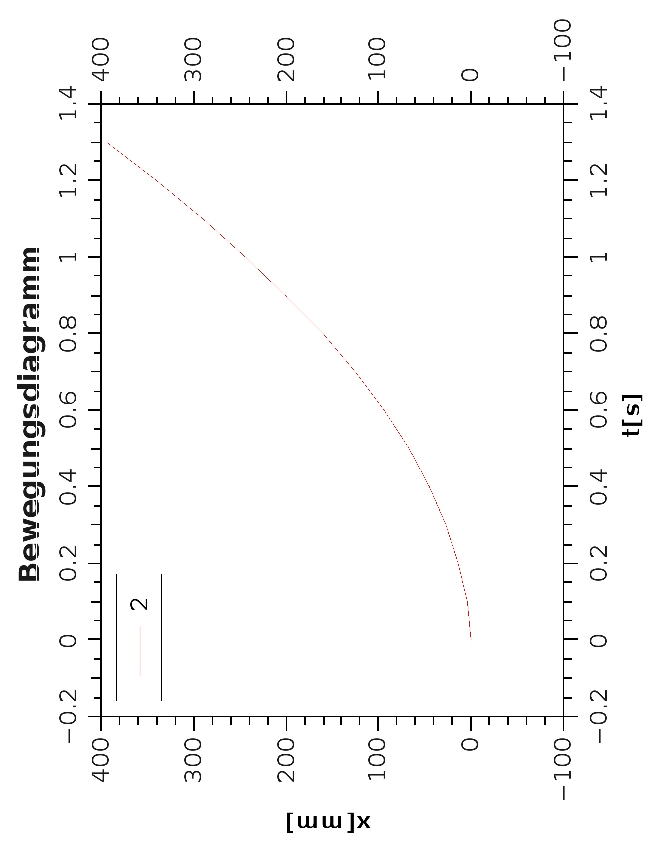
\includegraphics[scale=0.7,angle=-90]{glmbeschlBewegDiag.eps}
\end{center}
\end{figure}

\textbf{Regressionsanalyse}
\begin{figure}[H]
\caption{Geschwindigkeit}
\begin{center}
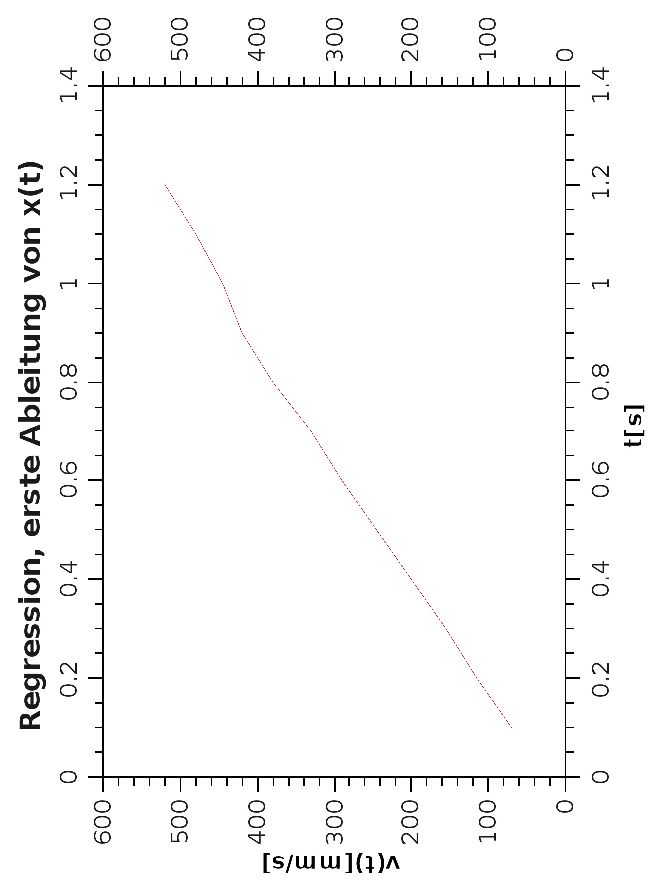
\includegraphics[scale=0.7,angle=-90]{RegressionGeschw.eps}
\end{center}
\end{figure}
\begin{figure}[H]
\caption{Beschleunigung}
\begin{center}
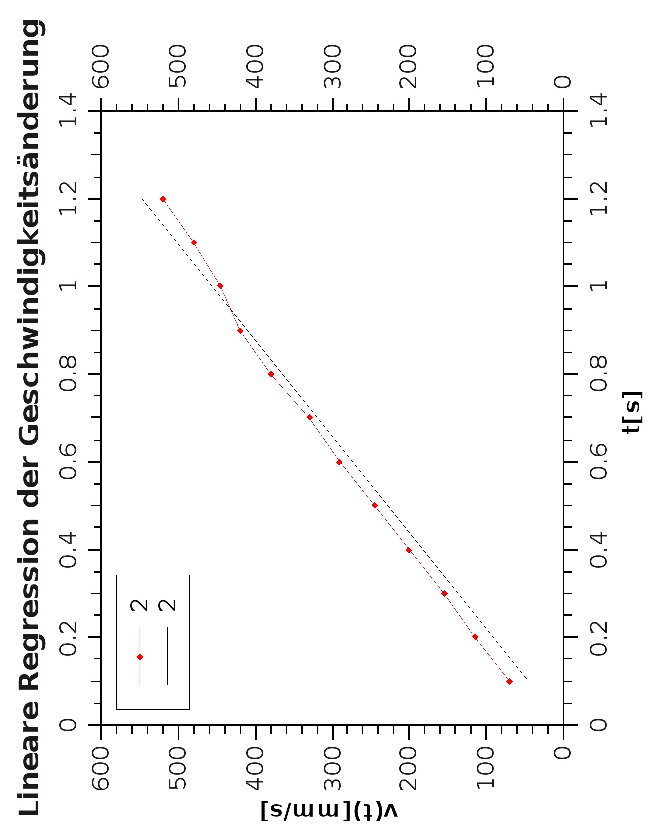
\includegraphics[scale=0.7,angle=-90]{GlmBeschlRegrBeschl.eps}
\end{center}
\end{figure}
Steigung der an der ersten Ableitung der Ortsfunktion gefitteten Gerade (also die Beschleunigung) 
A (slope) $\pm$ Err = 4.558461538461539e+02 +/- 7.598165175870181e+00
\begin{gather}
\vec{x}(t)=x_0+v_0t+\frac{1}{2}at^2 \\
A=\frac{1}{2}a \\
a=2A\pm Err=2\cdot 455.84 \pm 7.60=911.68\pm 7.60
\end{gather}

\textbf{Bewegungsgleichungen}

\textbf{Kraft}

\textbf{Gleitreibungskoeffizienten}


\subsection{Ergebnisse für die kräftefreie Bewegung}

\textbf{Schwerpunktgeschwindigkeit}

\textbf{Winkelgeschwindigkeit}

\textbf{Peripherie-Geschwindigkeitsvektor}


\subsection{Ergebnisse für den elastischen Stoß}

Wir beschweren den Gleiter 1 mit einem Gewicht von $\Delta$m=54.6g und führen die Stoßbewegung aus. Die beiden Gleiter sind gegeinander und leicht dezentral bewegt, mit annähernd konstanten Geschwindigkeiten.
\textbf{Geschwindigkeitsvektoren}

\textbf{Impulsvektoren}

\textbf{Überprüfung des Impulssatzes}

\textbf{Kinetische Energie}

\textbf{Schwerpunkt}


\subsection{Ergebnisse für den inelastischen Stoß}
Wir beschweren den Gleiter 1 mit einem Gewicht von $\Delta$m=54.6g und führen die Stoßbewegung aus.
\textbf{Geschwindigkeitsvektoren}

\textbf{Impulsvektoren}

\textbf{Überprüfung des Impulssatzes}

\textbf{Schwerpunkt}

\textbf{Kinetische Energie}


% ______________________________________Teil 2: Diskussion_____________________________________________


\subsection{Diskussion}
\textbf{Gleichmäßig beschleunigte Bewegung: Ermittelte und theoretisch wirkende Kraft}


\textbf{Kräftefreie Bewegung: }


\textbf{Elastischer Stoß: Diskussion der kinetischen Energie}

\textbf{Elastischer Stoß: Diskussion der Bahnkurve des Schwerpunktes}


\textbf{Inelastischer Stoß: Diskussion der Bahnkurve des Schwerpunktes}

\textbf{Inelastischer Stoß: Kinetische Energie}

\end{document}
